%%%%%%%%%%%%%%%%%%%%%%%%%%%%%%%%%%%%%%%%%%%%%%%%%%%%%%%%%%%%%%%%%
%
% Project     : Bachelorarbeit
% Title       : Machbarkeitsanalyse für eine ressourcenorientierte Schnittstelle zur Verarbeitung grundlegender Probleme der Informatik
% File        : umsetzung.tex Rev. 01
% Date        : 01.03.2015
% Author      : Raffael Santschi
%
%%%%%%%%%%%%%%%%%%%%%%%%%%%%%%%%%%%%%%%%%%%%%%%%%%%%%%%%%%%%%%%%%

\chapter{Umsetzung des Prototyps \resultAssignment{[R5]}}\label{chap.umsetzung}
In diesem Kapitel wird kurz auf die Erkenntnisse aus dem ersten Durchstich eingegangen. Danach wird erklärt, wie die Umsetzung für die ausgewählten Problemtypen schlussendlich 
durchgeführt wurde. Zu guter Letzt wird noch die Entwicklungsumgebung für dieses Projekt aufgezeigt.

\section{Erster Durchstich}\label{entwicklungsumgebung}
Zum Start der Umsetzung wurde ein erster \gls{vertikaler_durchstich} anhand des Rucksack Problems gemacht, um zu sehen, ob sich das Konzept bewährt. Während der 
Implementation wurden bereits überlegt, wie die Logik möglichst generisch gehalten werden kann.

\begin{figure}[h]
\centering
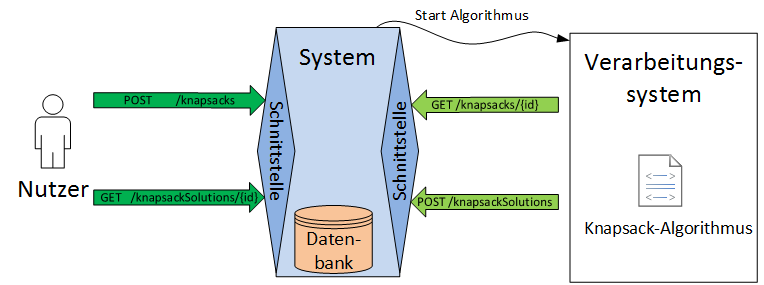
\includegraphics[scale=0.74]{images/visio/prototype_knapsack.png}
\caption[\Gls{vertikaler_durchstich} mit dem Rucksack Problem]{Vertikaler Durchstich mit dem Rucksack Problem \selfmade{}}
\label{fig:prototyp_knapsack}
\end{figure}

\subsection{Erkenntnisse nach dem ersten Durchstich}\label{learning_prototyp}
Die Kontaktschnittstelle nach Aussen generisch zu halten, macht aus Gründen der Benutzerfreundlichkeit keinen Sinn. Für den Kunden ist es transparenter, wenn er eine Schnittstelle aufruft, 
welche zum Beispiel 'timetabelScheduleComputations' heisst, als eine generische Schnittstelle, welche 'computations' heisst. Zudem ist nicht möglich, nur aus den Daten herauszufinden, was für 
ein Problem gelöst werden möchte. Dazu würde es einen zusätzlichen Parameter benötigen. Weiter stellt es sich in Java mit Spring als schwierig heraus, eine Endpunkt bereitzustellen, welcher 
verschiedene Ressourcentypen akzeptiert. Die Validierung der Eingabeparameter würde dadurch zusätzlich erschwert werden.

Das Konzept mit den beiden Translators bietet sehr viel Möglichkeiten und Flexibilität. Es entkoppelt die Nutzer-Schnittstelle komplett von der Schnittstelle für die Algorithmen. Um diese 
Flexibilität ausnutzen zu können, müssen jedoch oft verschiedene Entities für die Nutzer- und Algorithmus-Sicht erstellt werden.

In der Business Logik kann viel generisch gehalten werden. Die Repositories, Services und die Interfaces können generisch programmiert werden und bleiben für alle Probleme gleich. Beim 
Controller kann die Logik in einer abstrakten Klasse definiert werden und somit müssen nur noch die Namen der Schnittstellen in der spezifischen Implementation definiert werden. Es zeigte sich, 
dass sich das Konzept bewährt und die weiteren Probleme dementsprechend gelöst werden können.

\subsection{Anpassung des Konzepts nach dem ersten Durchstich}\label{doings_prototyp}
Das Konzept wurde nach dem ersten \glslink{vertikaler_durchstich}{Durchstich} dahingegen abgeändert, dass die Schnittstellen auf der Nutzer-Seite umbennant wurden und die Algorithmus-Seite einen anderen Namespace 
erhielt. Weiter verschwand die seperate Schnittstelle für das Abfrage des Resultats durch die Kombination mit der Status-Abfrage.

\section{Implementierung der Schnittstelle}\label{impl_interface}
In diesem Abschnitt wird über die Implementation der Schnittstelle im Allgemeinen geschrieben. Wie bereits erwähnt ist der Ablauf bei jedem Problem gleich, dementsprechend verhält sich die 
Schnittstelle im Allgemeinen gleich.

\subsection{Statusabfrage}
Damit der Nutzer möglichst wenig Schnittstellen ansprechen muss, erhält er bei einer Statusabfrage zugleich die vorhandenen Resultate. Der Nutzer erhält nur Resultate mit dem Status 'FINAL'. 
Resultate mit dem Status 'PARTIAL' werden zwar beim Status und der Zeit des zu letzt empfangenen Resultats berücksichtigt, aber nicht herausgegeben. Der Status besitzt neben den 
Resultaten, die ID und den Namen, weiter werden Start- und Endzeit angeben und zusätzlich noch die Zeit des zu letzt empfangenen Resultats. Falls eine Berechnung beendet ist, ist eine 
Begründung der Beendigung zu finden. Die Begründung kann zum Beispiel ein aufgetrettener Fehler während des Starts oder Berechnung sein.

\begin{lstlisting}[language=JSON, caption=Aufbau einer Antwort auf eine Statusabfrage, label=lst:status_response]  
{
  "id: "<Berechnung ID>",
  "name": "<Berechnungsname>",
  "computationStatus": "<Status der Berechnung>",
  "createDate": <Erstelldatum>,
  "finishDate": <Enddatum>,
  "finishedReason": "<Begruendung der Beendigung>",
  "lastResultReceived": <Datum des zu letzt empfangenen Resultats>,
  "solutions": <Resultate>
}
\end{lstlisting}

\subsection{WebHook Möglichkeit}
Die Berechnung können je nach Komplexität sehr lange dauern. Der Nutzer müsste immer wieder den Status abfragen, um zu sehen, ob ein Resultat vorhanden ist. \glspl{webhook} 
bieten Abhilfe für dieses Problem. Das Verfahren ist nicht standardisiert, ist aber sehr simpel und hilfreich. Beim Start einer Berechnung kann eine URL mitgegeben werden, zu dieser 
wird bei jeder Statusänderung ein POST-Request abgeschickt. Um diese Schnittstelle möglichst generisch zu halten, wurde eine Möglichkeit geschaffen, eine beliebige Payload für den 
POST-Request anzugeben. Die Nachricht des Statusänderung kann nach belieben mit dem Platzhalter '\_\_MESSAGE\_\_' irgendwo in die Payload eingebunden werden. Das Attribut 'message' 
wird in der Nachricht gesetzt, wenn der Platzhalter nirgends verwendet wird. Eine Konfiguraiton für die Chat Applikation 'Slack' würde wie in \autoref{lst:webhook_configuration} 
aussehen. Die Nachrichten bei den Statusänderungen sähen dann wie in \autoref{fig:slack_chat} aus.

\begin{lstlisting}[language=JSON, caption=Beispiel einer WebHook Konfiguration für Slack, label=lst:webhook_configuration]
  ...  
  "webHookConfiguration": {
    "url": "https://hooks.slack.com/services/T0000/B0000/XXX",
    "payload": {
        "text": "__MESSAGE__",
        "channel": "#simplatyser",
        "username": "simplatyser",
        "icon_emoji": ":squirrel:"
    }
  }
 ...
\end{lstlisting}

\begin{figure}[h]
\centering
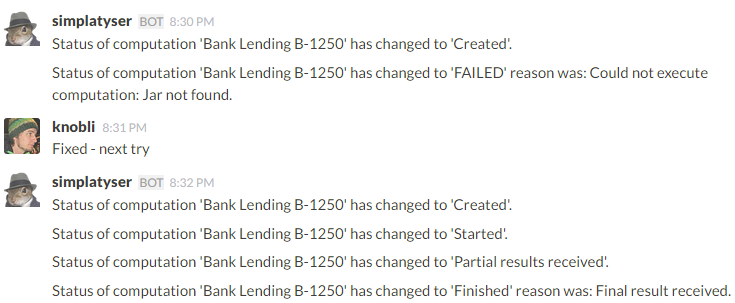
\includegraphics[scale=0.8]{images/slack_chat.png}
\caption[Nachrichten der Statusänderungen von Berechnungen]{Nachrichten der Statusänderungen von Berechnungen \selfmade{}}
\label{fig:slack_chat}
\end{figure}

\subsection{Technische Umsetzung und Probleme}
Das Fundament der Software war mit Spring-Boot \cite{spring_boot} sehr schnell gebaut, die Anbindung an die MongoDB wurde mit SpringData \cite{spring_data} realisiert. Leider waren 
oftmals die Dokumentationen nicht ausreichend oder nur für die XML-Konfiguration von Spring. Weiter gab es fehlende Teile in SpringData, welche herausgefunden werden mussten. 
So gibt es zum Beispiel zu diesem Zeitpunkt standardmässig keine Möglichkeit ein 'LocalTime'-Objekt oder ein 'LocalDateTime'-Objekt von Java 8 zu persistieren. Dies führte zu einem 
Stackoverflow anstatt einem Fehler, was wiederum die Suche nach dem Fehler erheblich erschwerte. Um diese Probleme zu beheben, musste ein eigener Converter geschrieben und dieser 
dann bei der MongoDB Konfiguration angegeben werden.

Bei der Business Logik wurde geschaut, dass viel mit \gls{generics} gelöst werden konnte, vorallem bei den Services konnte viel Code für alle Probleme verwendet werden. Auch 
bei den beiden Scheduling Problemen, konnte viel Code-Duplizierung umgangen werden. Zusätzlich wurden häufig verwendete Funktionen, wie das Abbilden auf die Input Objekte, in Helfer 
Klassen ausgelagert, damit sie nur ein Mal implementiert werden mussten.

\section{Implementierung der Probleme}\label{impl_problems}
In diesem Unterkapitel wird für jedes Problem kurz erklärt, was beim Prototyp implementiert wurde, um die Möglichkeiten des Konzepts aufzuzeigen. Eine ausführliche Schnittstellen 
Dokumentation ist in \autoref{api_doc} zu finden. Zusätzlich wurde noch eine elektronische Dokumentation der Schnittstelle mit Hilfe von Swagger UI erstellt, diese stellt die angebotenen 
Schnittstellen, die Eingabeparemter und Resultat sehr übersichtlich dar.

\begin{figure}[h]
\centering
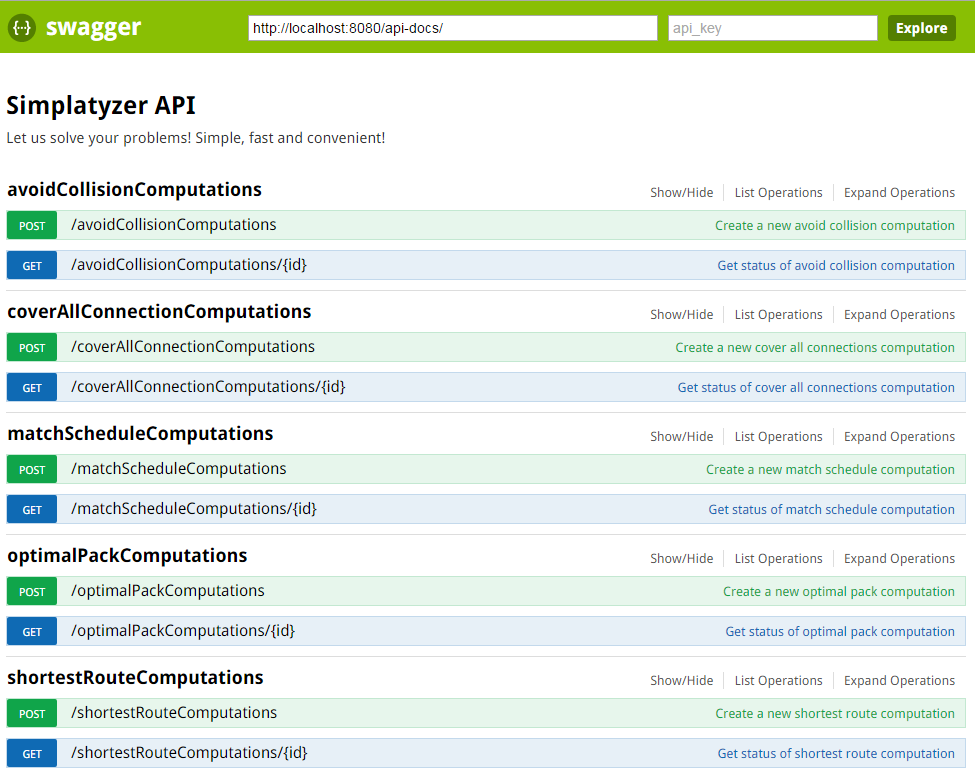
\includegraphics[scale=0.5]{images/swagger_api.png}
\caption[Nutzer Schnittstellenbeschreibung von Swagger]{Nutzer Schnittstellenbeschreibung von Swagger \selfmade{}}
\label{fig:swagger}
\end{figure}

\FloatBarrier

Beim Evaluieren des Stundenplan Problems wurde bemerkt, dass es sehr viele verschiedene Planungsprobleme gibt und deshalb wurde ein zusätzlich Planungsproblem gewählt, 
um zu schauen, wie sich die Schnittstelle bei sehr ähnlichen Problemen verhält.

%%%%%%%%%%%%%%%%%%%%%%%%%%%%%%%
%
%
%		Rucksack
%
%
%%%%%%%%%%%%%%%%%%%%%%%%%%%%%%%

\subsection{Rucksack}
Das Rucksack Problem ist aus Sicht der Schnittstelle ein relativ einfaches Problem. Aus Benutzerfreundlichkeit kann der Nutzer bei den Elementen eine Anzahl definieren und muss sie nicht 
doppelt angeben. Der Algorithmus hingegen bekommt eine Liste mit allen Elementen, es gibt nur noch einzelne Elemente und der Name wird nicht weiter gegeben, da er vom Algorithmus nicht 
benötigt wird. Der Algorithmus liefert als Resultat eine Liste von Boolean-Werten zurück, diese müssen zuerst wieder auf die eigentlichen Elemente abgebildet werden. Bei der Validierung wird 
überprüft, ob die Gewichtsschranke nicht überschritten wurde und ob ein Element nicht zu oft verwendet wurde. Letzeres ist zwar bei dem Test-Algorithmus nicht möglich, könnte jedoch bei 
einer anderen Implementation eventuell der Fall sein. Der Benutzer erhält als Resultat eine Liste mit allen Objekten, welche verwendet wurden. Wenn das Objekt mehrmals verwendet wurde, 
wird die entsprechende Anzahl angegeben.

\begin{figure}[h]
\centering
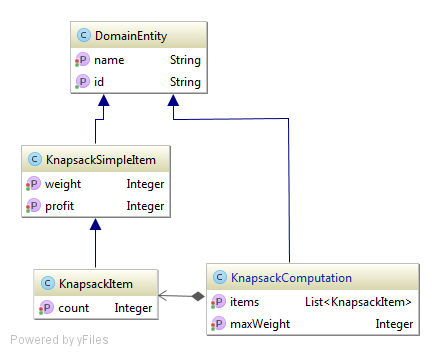
\includegraphics[scale=0.5]{images/probleme/knapsack.png}
\caption[Eingabeparameter für eine Rucksack Berechnung]{Eingabeparameter für eine Rucksack Berechnung \selfmade{}}
\label{fig:knapsack_input}
\end{figure}

\FloatBarrier

%%%%%%%%%%%%%%%%%%%%%%%%%%%%%%%
%
%
%		Knotenfärbung
%
%
%%%%%%%%%%%%%%%%%%%%%%%%%%%%%%%

\subsection{Knotenfärbung}
Beim Knotenfärbung geht es darum, Kollisionen zu vermeiden. Dies wurde für den Nutzer möglichst transparent umgesetzt. Der Nutzer kann mögliche Werte (z.B. Farben oder 
Frequenzen) angeben, welche die Element zugeteilt bekommen sollen. Der Algorithmus erhält eine Liste mit allen Elementen und ihren Nachbaren. Der Name der Elemente und die möglichen 
Werte werden nicht weiter gegeben. Es wird davon ausgegangen, dass der Algorithmus eine Liste von Elementen mit den zugewiesenen Werten zurückgibt. Beim Übersetzten werden, falls 
vorhanden, die Werte vom Algorithmus mit den möglichen Werten aus der Benutzereingabe ausgetauscht. Bei der Validierung wird überprüft, ob kein Element den gleichen Wert, wie einer 
seiner Nachbaren hat. Als Resultat erhält der Benutzer eine Liste mit allen Elementen und ihren zugewiesenen Werten.

\begin{figure}[h]
\centering
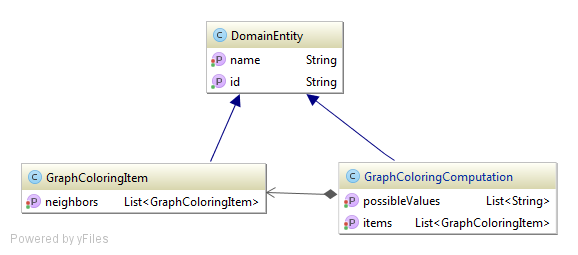
\includegraphics[scale=0.5]{images/probleme/graphcoloring.png}
\caption[Eingabeparameter für eine Knotenfärbung Berechnung]{Eingabeparameter für eine Knotenfärbung Berechnung \selfmade{}}
\label{fig:graphcoloring_input}
\end{figure}

%%%%%%%%%%%%%%%%%%%%%%%%%%%%%%%
%
%
%		Problem des Handlungsreisenden
%
%
%%%%%%%%%%%%%%%%%%%%%%%%%%%%%%%

\subsection{Problem des Handlungsreisenden}
Der Service bietet nicht nur die kürzeste Route für eine Liste von Wegpunkten an, es ist auch möglich für jeden Wegpunkt eine gewünschte Ankunftszeit und Aufenthaltszeit anzugeben. Der 
Nutzer kann eine Liste von Wegpunkten mit gewünschter Ankunftszeit und Aufenthaltszeit angeben. Der Algorithmus erhält vom System eine Liste mit allen Wegpunkten, bei diesem Schritt wird 
nichts übersetzt. Es wäre möglich, dass die Schnittstelle bereits die Distanzen zwischen den Wegpunkten berechnet oder die Daten sonst irgendwie für den Algorithmus aufbereitet. Es 
wird davon ausgegangen, dass der Algorithmus eine Liste von den Wegpunkten in der berechneten Reihenfolge zurückgibt. Beim Übersetzten werden die geplanten Ankunftszeiten berechnet, 
welche dann während der Validierung mittels der maximal angegebenen Abweichung überprüft werden. Der Benutzer erhält als Resultat eine Liste mit der berechneten Reihenfolge der 
Wegpunkte und jeder Wegpunkt besitzt die gewünschte und geplante Ankunftszeit.

\begin{figure}[h]
\centering
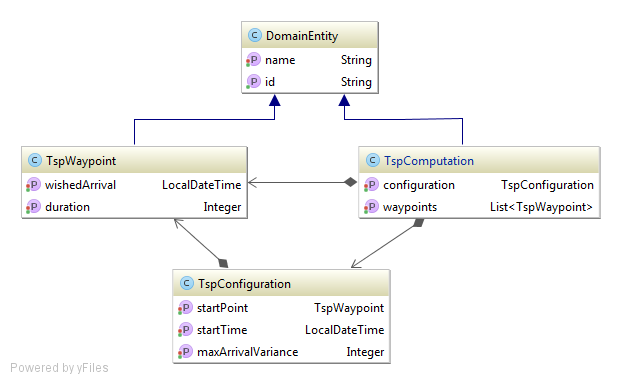
\includegraphics[scale=0.5]{images/probleme/tsp.png}
\caption[Eingabeparameter für eine Routen Berechnung]{Eingabeparameter für eine Routen Berechnung \selfmade{}}
\label{fig:tsp_input}
\end{figure}

%%%%%%%%%%%%%%%%%%%%%%%%%%%%%%%
%
%
%		Briefträgerproblem
%
%
%%%%%%%%%%%%%%%%%%%%%%%%%%%%%%%

\subsection{Briefträgerproblem}
Das Briefträgerproblem berechnet eine Route, welche alle bekannten Wege einer Strecke abfährt. Der Nutzer kann eine Liste von Wegpunkten mit den bekannten Verknüpfungen zu anderen 
Wegpunkten und ihrer Dinstanz angeben. Der Algorithmus erhält vom System eine Liste mit allen Wegpunkten, die Namen der Wegpunkte werden nicht weitergegeben. Es wird davon ausgegangen, 
dass der Algorithmus eine Liste von den Wegpunkten in der berechneten Reihenfolge zurückgibt. Beim Übersetzten werden die Wegpunkte wieder auf die Eingabewerte abgebildet und die komplette 
Länge der Route berechnet. Die Validierung überprüft, ob der Weg möglich ist und ob jede Verbindung ein Mal benutzt wurde. Der Benutzer erhält als Resultat eine Liste mit der berechneten 
Reihenfolge der Wegpunkte und die totale Länge der Strecke.

\begin{figure}[h]
\centering
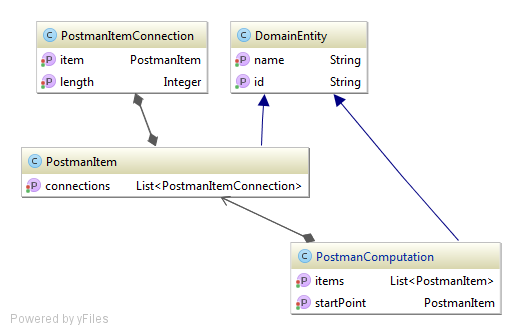
\includegraphics[scale=0.5]{images/probleme/postman.png}
\caption[Eingabeparameter für eine Briefträger Routen Berechnung]{Eingabeparameter für eine Briefträger Routen Berechnung \selfmade{}}
\label{fig:postman_input}
\end{figure}

%%%%%%%%%%%%%%%%%%%%%%%%%%%%%%%
%
%
%		Stundenplan Erstellung
%
%
%%%%%%%%%%%%%%%%%%%%%%%%%%%%%%%

\subsection{Stundenplan Erstellung}
Das Erstellen eines Stundenplans ist ein Planungsproblem, welches sehr vielen Möglichkeiten und Einschränkungen besitzt und somit sehr komplex ist. In dieser Implementation sind bei weiten 
nicht alle Spezialitäten abgedeckt. Es wurde geschaut, dass bereits einige Einschränkungen, wie zum Beispiel freie Tage von Lehrern und blockierte Schulzimmer, miteinbezogen werden. 
Der Nutzer gibt eine Liste von Klassen, Lehrern, Schulzimmern und Schulfächern an. Die Klassen haben eine Grösse und definieren auch, welche Fächer sie besuchen müssen. Die Lehrer haben 
eine Liste mit Schulfächern, welche sie unterrichten können, eine List mit zugehörigen Klassen und eine Definition ihrer freien Tage. Die Klassenzimmer besitzen eine Liste mit möglichen 
Schulfächern und eine Sperrlist, in welcher definiert ist, wann der Raum nicht verfügbar ist. Die Schulfächer können definieren, ob sie eine Raum brauchen, welcher explizit dafür 
bestimmt ist, zum Beispiel Sport in der Turnhalle. Neben den Elementen, welche verplant werden, gibt es Randbedingungen wie die Pausenzeiten, die Lektionsdauer und die Definition, 
wann unterrichtet werden soll. Der Algorithmus erhält eine Liste mit allen Klassen, Lehrern, Schulzimmern und Schulfächern. Die Rahmenbedingungen werden in Zeitschlitze umgewandelt, 
welche vom Algorithmus verplant werden können. Zusätzlich werden die Elemente generischer benannt, damit der Algorithmus nicht verschiedene Konfigurationen für verschiedene 
Planungsprobleme besitzen muss. In \autoref{lst:cat_input_timetableScheduling} ist ein Beispiel für eine Eingabe der Rahmenbedingungen gezeigt, welche durch den Translator in die 36 Zahl 
umgewandelt werden würde. Die Zahl wird aus der Lektionsdauer, den Pausen und den einzelnen Zeitfenstern pro Tag berechnet, die \autoref{table:timeslice_calc} stellt dies visuell dar.

\begin{lstlisting}[language=JSON, caption=Ausschnitt einer Eingabe für das Stundenplanproblem für die Rahmenbedingungen, label=lst:cat_input_timetableScheduling]  
{
  ...
  "configuration": {
    "breakTimeSliceSize": [5, 20, 5, 90, 5, 20, 5],
    "dayTimeSlots": [
      {
        "monday": {"defaultTimes": true},
        "tuesday": {"defaultTimes": true},
        "wednesday": {"from": [8, 20, 0], "to": [12,0,0]},
        "thursday": {"defaultTimes": true},
        "friday": {"defaultTimes": true}
      }
    ],
    "lessonDuration": 45
  }
}
\end{lstlisting}

\begin{table}[ht]
\centering
  \begin{tabular}{ l | c | c | c | c | c }
	\hline
	\rowcolor{gray}
	\textbf{Uhrzeit} 	& \textbf{Mo}	& \textbf{Di} 	& \textbf{Mi}	&  \textbf{Do}	&  \textbf{Fr}\\ \hline
	0820-0905		& 1			& 9			& 17			& 21			& 29		\\ \hline
	0910-0955		& 2			& 10			& 18			& 22			& 30		\\ \hline
	1015-1100		& 3			& 11			& 19			& 23			& 31		\\ \hline
	1105-1150		& 4			& 12			& 20			& 24			& 32		\\ \hline \hline
	1320-1405		& 5			& 13			& -			& 25			& 33		\\ \hline
	1410-1455		& 6			& 14			& -			& 26			& 34		\\ \hline
	1515-1600		& 7			& 15			& -			& 27			& 35		\\ \hline
	1605-1650		& 8			& 16			& -			& 28			& 36		\\ \hline
  \end{tabular}
   \caption{Visuelle Darstellung der Zeitfenster Berechnung}\label{table:timeslice_calc}
\end{table}

\begin{figure}[h]
\centering
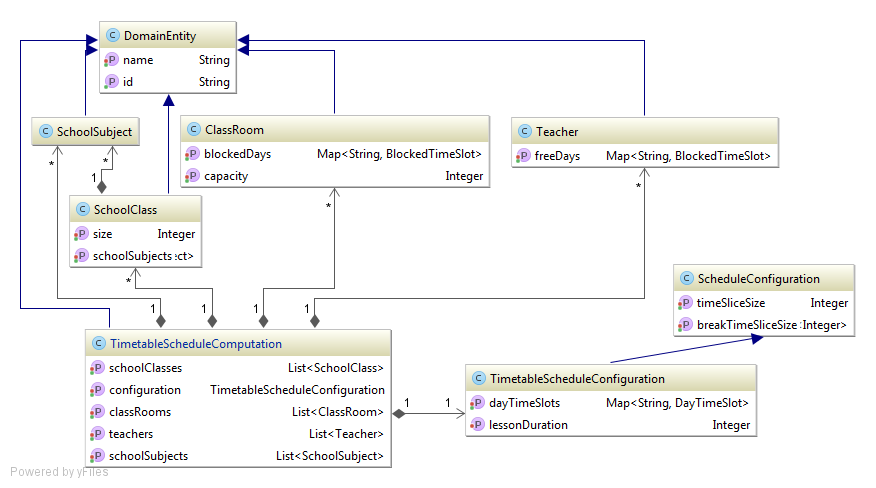
\includegraphics[scale=0.5]{images/probleme/timetableSchedule.png}
\caption[Eingabeparameter für eine Stundenplan Berechnung]{Eingabeparameter für eine Stundenplan Berechnung \selfmade{}}
\label{fig:timetableSchedule_input}
\end{figure}

\FloatBarrier

Es wird davon ausgegangen, dass der Algorithmus eine Liste von Planungskombinationen zurück gibt. Eine Kombination besteht aus einer Zeitfensternummer, einem Lehrer, einer Klasse, 
einem Schulfach und einem Klassenzimmer. Beim Übersetzten werden die IDs auf die ursprünglichen Elemente abgebildet und die Zeitfensternummern werden in Uhrzeiten umgewandelt. 
Zusätzlich wird eine Statistik für die Lehrer geführt. Bei der Validierung wird geschaut, ob ein Element zu einer Zeit zwei Mal verplant ist, ob der Lehrer die nötigen Fähigkeiten hat und ob ein 
Klassenzimmer für das Fach ausgelegt ist. Das Resultat für den Nutzer enthält eine Liste mit den berechneten Kombination, sortiert nach Wochentag und Uhrzeit. Die Lehrerstatistik zeigt, wie 
oft ein Lehrer ein bestimmtes Fach unterrichtet und wie viel Stunden er insgesamt unterrichtet.

%%%%%%%%%%%%%%%%%%%%%%%%%%%%%%%
%
%
%		Spielplan Erstellung
%
%
%%%%%%%%%%%%%%%%%%%%%%%%%%%%%%%

\subsection{Spielplan Erstellung}
Eine weitere Ausprägung des Planungsproblem ist das Erstellen eines Spielplans. Der Nutzer gibt eine Liste von Teams, Schiedsrichter, Spielfelder und Kategorien an. Die Teams haben eine 
bestimmte Kategorie. Die Schiedsrichter haben eine Liste mit Kategorien, welche sie leiten können und eine Liste von Teams, zu welchen sie gehören. Die Spielfelder besitzen eine Liste mit 
möglichen Kategorien. Neben den Elementen, welche verplant werden, gibt es Randbedingungen wie die Spieldauer, der Starzeit und die Pausenzeiten. Der Algorithmus erhält eine 
Liste mit allen Teams, Schiedsrichter, Spielfelder und Kategorien. Zusätzlich werden die Elemente generischer benannt, damit der Algorithmus nicht verschiedene Konfigurationen für 
verschiedene Planungsprobleme besitzen muss.

\begin{figure}[h]
\centering
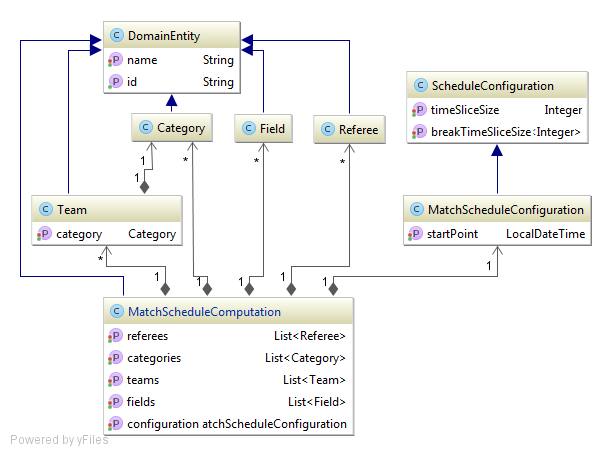
\includegraphics[scale=0.5]{images/probleme/matchSchedule.png}
\caption[Eingabeparameter für eine Spielplan Berechnung]{Eingabeparameter für eine Spielplan Berechnung \selfmade{}}
\label{fig:matchschedule_input}
\end{figure}

Es wird davon ausgegangen, dass der Algorithmus eine Liste von Planungskombinationen zurück gibt. Eine Kombination besteht aus einer Zeitfensternummer, einem Schiedsrichter, 
einer Kombination von zwei Teams und einem Spielfeld. Beim Übersetzten werden die IDs auf die ursprünglichen Elemente abgebildet und die Zeitfensternummern werden in Uhrzeiten 
umgewandelt. Zusätzlich wird eine Statistik für die Schiedsrichter und die Teams geführt, wie viele Einsätze sie jeweils haben. Bei der Validierung wird geschaut, ob ein Element zu einer Zeit zwei 
Mal verplant ist, ob die Schiedsrichter die nötigen Fähigkeiten haben und ob ein Spielfeld für die Kategorie ausgelegt ist. Der Benutzer erhält als Resultat eine Liste mit den berechneten 
Kombination, sortiert nach Uhrzeit. Die Schiedsrichterstatistik zeigt, wie oft ein Schiedsrichter eine bestimmte Kategorie pfeifft und für wie viel Spiele er insgesamt verantwortlich ist. Die 
Teamstatistik zeigt, wie viele Spiele eine Kategorie insgesamt hat und wie viele Spiele ein Team bestreitet. In \autoref{lst:cat_result_matchScheduling} wird eine Ausschnitt der 
Schiedsrichterstatistik dargestellt.

\begin{lstlisting}[language=JSON, caption=Ausschnitt eines Resultats einer Spielplan Erstellung, label=lst:cat_result_matchScheduling]  
{
  ...
  name: "Sabine Pfister"
  statisticMap: {
    Knaben: 1
    Damen Kat A: 3
    Damen Kat B: 2
    _TOTAL: 6
  }
  ...
}
\end{lstlisting}

\subsection{Übersicht der Schnittstellen}
Für den Nutzer wurde ein Problem agnostischer Namen für die Schnittstelle gewählt. Die Namen unterscheiden sich somit zum Teil zwischen Nutzer- und Algorithmus-Sicht voneinander. Damit die 
Verknüpfung der beiden Schnittstellen nicht verloren geht und eine Übersicht über alle angebotenen Schnittstellen zu haben, wurden sie in der \autoref{table:overview_api_interfaces} 
zusammengetragen. Die Schnittstellen für die Algorithmen sind unter einem anderen Namespace '/algorithm', damit diese sauber voneinander getrennt sind.

\begin{table}[ht]
\centering
  \begin{tabular}{ l | l }
	\hline
	\rowcolor{gray}
	\textbf{Nutzer}							& \textbf{Algorithmus}					\\ \hline
	/									& /algorithm/							\\ \hline
	\multicolumn{2}{|c|}{\textbf{Allgemein}}\\ \hline
	 Berechnung starten				& Berechnungsinformationen abholen			\\ \hline
	Status bzw. Lösung	abholen & Lösung bekannt geben	\\ \hline
	\multicolumn{2}{|c|}{\textbf{Rucksack}}\\ \hline
	 POST /optimalPackComputations					& GET /knapsackComputations/\{ID\}			\\ \hline
	GET /optimalPackComputations/\{ID\}	& POST /knapsackComputations/\{ID\}/solutions	\\ \hline
	\multicolumn{2}{|c|}{\textbf{Knotenfärbung}}\\ \hline
	POST /avoidCollisionComputations				& GET /graphColoringComputations/\{ID\}		\\ \hline
	GET /avoidCollisionComputations/\{ID\}		& POST /graphColoringComputations/\{ID\}/solutions	\\ \hline
	\multicolumn{2}{|c|}{\textbf{Problem des Handlungsreisenden}}\\ \hline
	POST /shortestRouteComputations				& GET /tspComputations/\{ID\}				\\ \hline
	GET /shortestRouteComputations/\{ID\}		& POST /tspComputations/\{ID\}/solutions		\\ \hline
	\multicolumn{2}{|c|}{\textbf{Briefträgerproblem}}\\ \hline
	POST /coverAllConnectionComputations				& GET /postmanComputations/\{ID\}			\\ \hline
	GET /coverAllConnectionComputations/\{ID\} 	& POST /postmanComputations/\{ID\}/solutions	\\ \hline
	\multicolumn{2}{|c|}{\textbf{Stundenplan Erstellung}}\\ \hline
	POST /timetableComputations				& GET /timetableComputations/\{ID\}			\\ \hline
	GET /timetableComputations/\{ID\}	& POST /timetableComputations/\{ID\}/solutions	\\ \hline
	\multicolumn{2}{|c|}{\textbf{Spielplan Erstellung}}\\ \hline
	POST /matchesScheduleComputations				& GET /matchesScheduleComputations/\{ID\}			\\ \hline
	GET /matchesScheduleComputations/\{ID\}	& POST/matchesScheduleComputations/\{ID\}/solutions	\\ \hline
  \end{tabular}
   \caption{Übersicht der angebotenen Schnittstellen}\label{table:overview_api_interfaces}
\end{table}

\FloatBarrier

\subsection{Erstellung eines neuen Problems}
Das Ziel dieser Arbeit war die Erstellung einer Schnittstelle, welche einfach zu erweitern ist. Dieser Abschnitt soll zeigen, wie dies erreicht wurde und wie sie erweitert werden kann. Das 
Software Projekt ist in Packages gegliedert. Auf der ersten Ebenen befinden sich die generischen Klassen und die spezifischen Implementierung sind unter dem Package 'problem'  angesiedelt. 
Die Gliederung ist so gewählt, damit ein Problem nur an einem Ort im Projekt verhängt ist und nicht an vielen verschiedenen Stellen gesucht werden muss. Es wäre möglich, 
die verschiedenen Problem-Implementationen in ein anderes Projekt auszulagern.

Um ein neues Problem in den Katalog aufzunehmen, 
müsste ein neues Package mit dem Problemnamen erstellt werden. Darin sind weitere Packages zur besseren Übersicht definiert. Als erstes müsste das Problem analysiert werden und 
dementsprechend die Entities für die Eingabe und das Resultat bereit gestellen werden.

Sind die Entities definiert, muss ein Controller für den Algorithmus und einer für den Nutzer erstellt werden. Die Controller leiten von einer abstrakten Klasse ab und dienen lediglich zur Definition
der neuen Endpunkte. Die Dokumentation der Controller wird auch im den jeweiligen Klassen geschrieben, dies erweitert automatisch die elektronische Dokumentation von Swagger UI. 
Nun fehlen noch die beiden Translator für das Umwandeln der Nutzer-Sicht in die Algorithmus-Sicht, der Validator für das Problem und der Solver, welcher den Algorithmus 
startet. Alles andere ist generischer Code, welcher nur noch mit den jeweiligen Entity-Typen spezifiziert werden muss.

Zu guter Letzt wird noch ein Beispiel für eine Eingabe aus Nutzer-Sicht und ein Resultat aus Algorithmus-Sicht in JSON unter den Ressourcen abgelegt. Diese Beispiele können für Tests 
verwendet werden.

\newpage

\section{Entwicklungsumgebung}\label{entwicklungsumgebung}
Ein Softwareprojekt benötigt immer eine gewisse Entwicklungsumgebung. Bei der Entwicklung mit Spring-Boot sind die Anfoderungen minimal, da Spring-Boot bereits einen eigenen Webserver 
mitbringt.

\subsection{IDE - Integrated Development Environment}
Als \gls{ide} wurde IntelliJ verwendet, IntelliJ bietet gute Refactoring-Methoden an und ist eine grosse Unterstützung beim Programmieren von Java-Code. Die \gls{ide} 
bietet auch die Möglichkeit Klassen-Diagramme zu erstellt und hat ein \gls{vim}-Plugin. Mit diesem Plugin können \gls{vim}-Befehle benutzt werden, was die 
Geschwindigkeit beim Programmieren enorm erhöht.

\todo{Ausschnitt aus Intellij, welcher gleich die Struktur des Projekts zeigt}

\subsection{Versionierung}
Für die Versionierung der Software wurde git \cite{git} verwendet. Das Remote Repository wurde auf Github \cite{github_simplatyzer} erstellt. Es wurde darauf geachtet, dass 
der Code oft ins Repository geladen wurde, damit ein Backup existiert. Die Dokumentation wurde in Dropbox gespeichert, damit auf verschiedenen Computern darauf zu gegriffen werden konnte 
und immer ein Backup vorhanden war. Zu Korrekturzwecken wurde die Arbeit ebenfalls auf github hochgeladen und die Änderungsvorschläge wurden mit Latexdiff verglichen.

\begin{figure}[h]
\centering
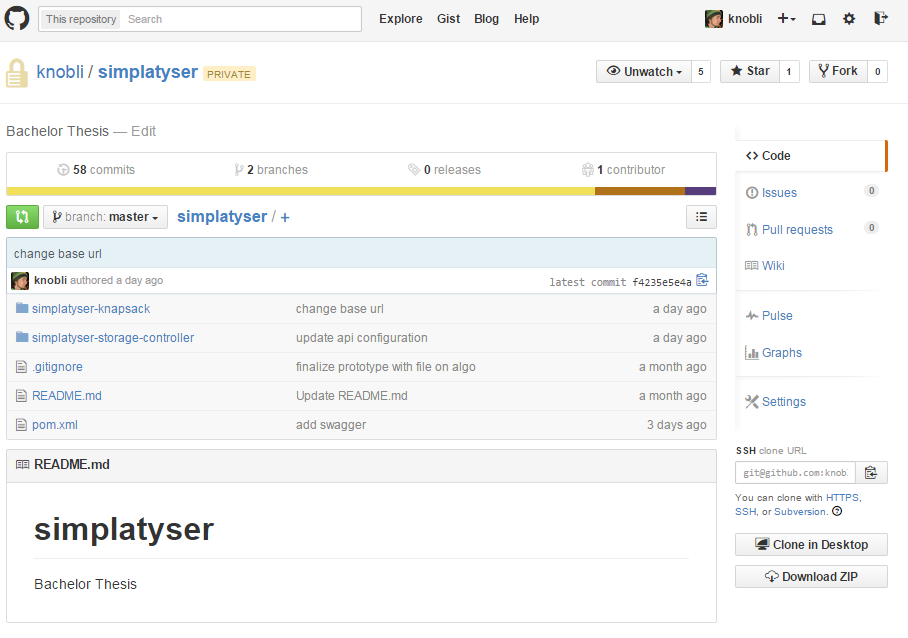
\includegraphics[scale=0.5]{images/github.png}
\caption[Github Repository des Simplatyser Projekts]{Github Repository des Simplatyser Projekts \selfmade{}}
\label{fig:github_repo}
\end{figure}

\subsection{Testen - Analysieren}
 Über den Chrome App 'Advanced REST client' (siehe Abbildung \ref{fig:advanced_rest_client})  wurde die Schnittstelle manuell getestet. Für die Regression-Tests wurde Junit und Mockito 
verwendet. Die statische Code Analyse wurde mit \gls{sonar} \cite{sonar} durchgeführt.

\begin{figure}[h]
\centering
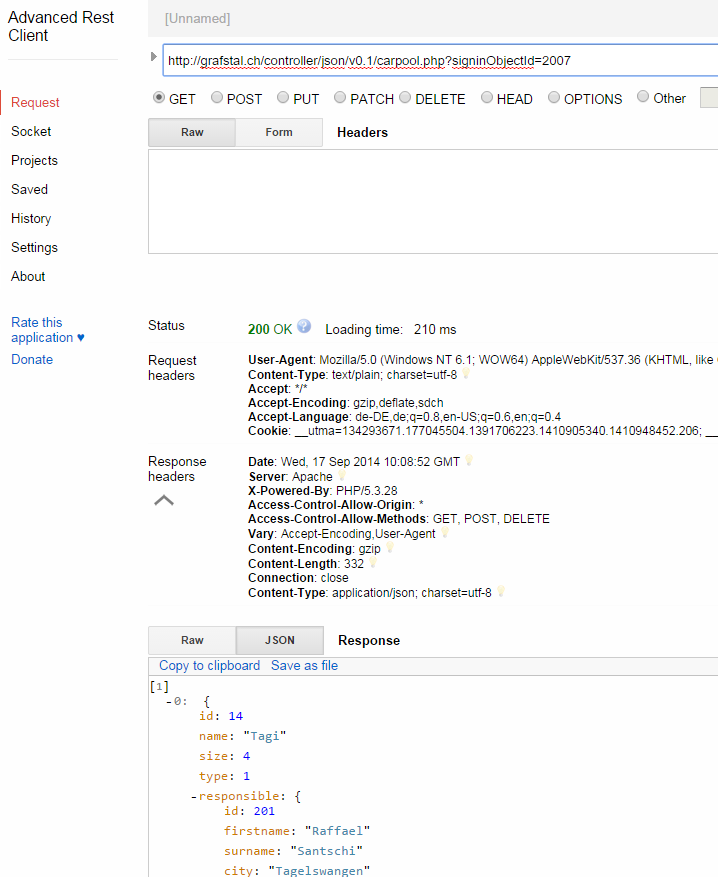
\includegraphics[scale=0.7]{images/advanced_rest_client.png}
\caption[Advanced Rest client]{Advanced Rest client \selfmade{}}
\label{fig:advanced_rest_client}
\end{figure}